\documentclass[a4paper,12pt]{report}
%general packages
\usepackage[T2A]{fontenc}
\usepackage[utf8]{inputenc}
\usepackage[english,russian]{babel}
\usepackage{circuitikz}
\usepackage{wrapfig}
\usepackage{makecell}
\usepackage{tabularx}
\usepackage{graphicx}
\usepackage{gensymb}
\usepackage{cancel} %cancel symbol
\usepackage{amsmath,amsfonts,amssymb,amsthm,mathtools}
\usepackage[dvipsnames]{xcolor}

%fancy header + geometry
\usepackage{fancyhdr}
\usepackage[a4paper,includehead,nomarginpar,left=15mm,right=15mm,top=15mm,headheight=10mm,bottom=20mm]{geometry}

%pgfplots
\usepackage{pgfplots}
\usepackage{pgfkeys}
\pgfplotsset{compat=1.12}
\usepackage{mathrsfs}

%multi column text
\usepackage{blindtext}
\usepackage{multicol}

%tikz (draw)
\usepackage{tikz}
\usepackage{pstricks-add}
\usetikzlibrary{intersections}
\usetikzlibrary{arrows.meta}
\usetikzlibrary{calc,angles,positioning}
\usetikzlibrary{arrows}
\usepackage{float}

%parskip settings
\parindent=0ex
\setlength{\parskip}{\baselineskip}%
\setlength{\parindent}{0pt}%

%fancy notation for sets
\newcommand{\R}{{\mathbb R}}
\newcommand{\N}{{\mathbb N}}
\newcommand{\fancy}[1]{{\mathbb{#1}}}
%sgn function
\DeclareMathOperator{\sgn}{sgn}

% intersection and union symbols
\newcommand{\uni}{\cup}
\newcommand{\inter}{\cap}
\newcommand{\re}{\text{Re}}
\newcommand{\const}{\text{const}}

\renewcommand{\footrulewidth}{0.4pt}

%\newcommand{\celsius}{$\ ^\circ C$}

%environments

\newtheorem{problem}{Задача}[]
\newenvironment{sol}{\paragraph{Решение}}{}
\renewcommand\thesection{\arabic{section}}

\usepackage{titlesec}
\titlespacing*{\section}
{0cm}{\baselineskip}{0pt}
\titlespacing*{\subsection}
{0pt}{0.1\baselineskip}{0.1\baselineskip}
\titlespacing*{\paragraph}
{0pt}{0.1\baselineskip}{\baselineskip}

\setcounter{secnumdepth}{0}

\begin{document}
	

\begin{titlepage}
	\begin{center}
		МОСКОВСКИЙ ФИЗИКО-ТЕХНИЧЕСКИЙ ИНСТИТУТ (НАЦИОНАЛЬНЫЙ ИССЛЕДОВАТЕЛЬСКИЙ УНИВЕРСИТЕТ) \\
		
		
		\hfill \break
		Факультет обшей и прикладной физики\\
		\vspace{2.5cm}
		\large{\textbf{Отчёт по лабораторной работе 1.2.5 <<Исследование прецессии уравновешенного гороскопа>>}}\\
		\hfill \break
		\\
	\end{center}
	
	\begin{flushright}
		Выполнил:\\
		Студент гр. Б02-304\\
		Головинов. Г.А.
	\end{flushright}
	
	\vspace{7cm}
	
	\begin{center}
		
\includegraphics[width=0.15\linewidth]{uni}
	\end{center}
	

	

	\vfill
	
	\begin{center} Долгопрудный, 2023 \end{center}
	
	\thispagestyle{empty}
	
\end{titlepage}


	\newpage
	%\pagenumbering{arabic}
    \pagestyle{fancy}

    \fancyhead{}
    \fancyfoot{}
    \fancyhead[L]{\rightmark}
    \fancyhead[R]{\thepage}
    \fancyfoot[R]{Работа 2.5.1. --- Определение коэффициента поверхностного натяжения в зависимости от температуры}

    \section*{Аннотация}
        \paragraph*{Цель работы:} 1) измерить коэффициент поверхностного натяжения в зависимости от температуры; 2) определение полной поверхностной энергии и теплоты, необходимой для изотермического образования единицы поверхности жидкости.
        \paragraph*{В работе используются:} прибор Ребиндера с термостатом; исследуемые жидкости; стаканы; линейка.
    \vspace{0.5cm}
    \hrule

    \begin{multicols}{2}
        \section{Основные теоретические сведения.}
        Рассмотрим пузырь воздуха в некоторой жидкости. Если он имеет сферическую форму и радиус $r$, то внутри него давление на $\Delta p$ выше, чем в жидкости. $\Delta p$ находится из следующего соотношения, которое называется формулой Лапласа:
        \begin{equation}
            \Delta p = \frac{2\sigma}{r}
        \end{equation}
        Определять коэффициент поверхностного натяжения будем как раз с помощью нее: зная разницу давления и радиус иглы (который можно измерить двумя способами: прямо и косвенно) мы можем найти искомый коэффициент. В работе предлагается исследовать зависимость коэффициента поверхностного натяжения от температуры жидкости.
        \paragraph*{Термодинамика поверхностного натяжения.}
        Из первого начала термодинамики и определения коэффициента $\sigma$:
        \begin{equation*}
            \delta Q = dU_\Pi - \sigma d\Pi
        \end{equation*}
        где $dU_\Pi$ --- полная поверхностная энергия. Далее запишем через энтропию:
        \begin{equation}
            dU_\Pi = TdS+\sigma d\Pi
            \label{dU}
        \end{equation}
        Перейдем к свободной энергии $F$, которая по определению:
        \begin{equation}
            F=U_\Pi-TS
        \end{equation}
        Подставляя \eqref{dU} в предыдущее выражение получим:
        \begin{equation}
            dF=-SdT+\sigma d\Pi
        \end{equation}
        Откуда
        \begin{equation}
            \label{double}
            S=-\left(\frac{\partial F}{\partial T}\right)_\Pi, \qquad \sigma = \left(\frac{\partial F}{\partial \Pi}\right)_T.
        \end{equation}
        Последнее можно проинтегрировать, учитывая как граничные условия, что $F=0$ при $\Pi = 0$. Получим:
        \begin{equation}
            F=\sigma\Pi
        \end{equation}
        Это можно подставить в первое из двух соотношений в \eqref{double} и получить
        \begin{equation*}
            S=-\Pi \frac{d\sigma}{dT}
        \end{equation*}
        Тогда получим выражение для энергии:
        \begin{equation}
            U_\Pi=\left(\sigma-T\frac{d\sigma}{dT}\right)\Pi
        \end{equation}
        При изотермическом процессе полная энергия увеличивается только из-за увеличения площади поверхности, при этом к ней нужно подвести тепло
        \begin{equation*}
            Q=\Delta U_\Pi - \sigma \Delta \Pi = -T\frac{d\sigma}{dT}\Delta\Pi
        \end{equation*}
        На единицу площади:
        \begin{equation*}
            q=-T\frac{d\sigma}{dT}
        \end{equation*}
        А энергия на единицу площади:
        \begin{equation*}
            \frac{\Delta U_\Pi}{\Delta\Pi}=q+\sigma
        \end{equation*}
        \newcolumn
        \section{Экспериментальная установка.}
        \begin{figure}[H]
            \centering
            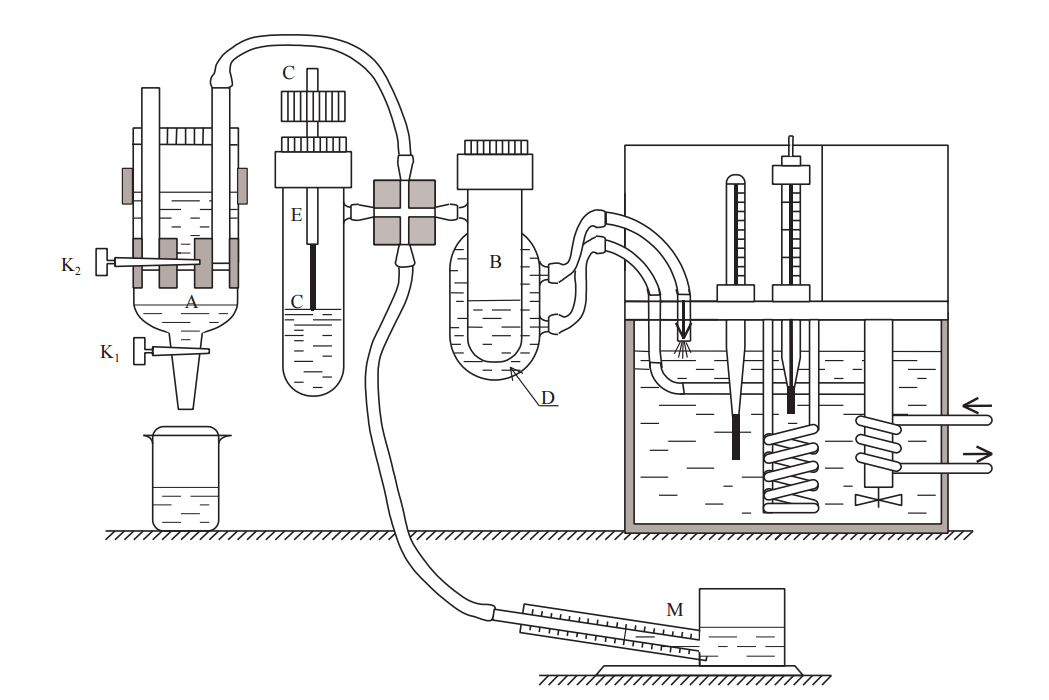
\includegraphics[width=\columnwidth]{../img/ustanovka.png}
            \caption{Схема установки}
        \end{figure}
        Температура исследуемой жидкости (воды) поддерживается установленной с помощью термостата. Когда мы открываем кран К$_1$, из аспиратора А вытекает вода. Это создает падение давления внутри системы, которое можно измерить манометром М.

        Верхний конец иглы открыт, внутри иглы атмосферное давление $p_0$. Так как давление в системе $p'<p_0$, на конце игры начинает образовываться пузырь. Давление внутри пузыря остается атмосферным, значит внутри системы новое давление $p_0-\Delta p=p_0-2\sigma/r$. Манометр измеряет разницу давления внутри системы и атмосферы, причем в этом случае он будет показывать давление внутри пузыря.

        Если мы находимся на глубине $h$ под поверхностью жидкости, то давление в жидкости на этом же уровне будет $\rho g h -2\sigma/r$, на поверхности и в системе тогда $p_0-2\sigma/r$. Поэтому максимальное показание манометра и есть добавочное давление $\Delta p$. Максимальным оно будет в момент, когда радиус пузырька равен радиусу иглы. Поэтому нас интересует именно максимальное давление.
        \newcolumn
        \section{Обработка результатов.}
        По полученным точкам (см. таблицы в приложении) построим зависимость $\sigma(T)$, аппроксимируем ее по методу МНК прямой $y=kx+b$. Наклон этой прямой $d\sigma/dT$ можно будет сравнить с табличным (так же как и сами значения $\sigma$).

        Погрешность $\delta T$ примем за $0.2$ K, так как термостат часто <<перескакивал>> заданные значения на несколько долей градуса. Погрешность коэффициента поверхностного натяжение складывается из приборной и случайной составляющей.
        
        Приборная обусловлена погрешностью измерения с помощью манометра, положим $\delta_p=0.5$ делений, что равно $\approx 1 \ \text{Pa}$. Кроме того в приборную погрешность входит погрешность измерения высоты: 0.5 mm. Оценим каждое значение максимальной погрешностью. Итого $\delta_\text{приборная}\approx 0.6 \ \text{mN}/\text{m}$.

        Для оценки случайной погрешности мы провели по 5 измерений для каждой температуры. Посчитаем стандартное отклонение:
        \begin{equation*}
            \delta_\text{случайная}=\sqrt{\frac{1}{n-1}\sum_{i=1}^{n}(x_i-\langle x \rangle)^2}
        \end{equation*}
        Некоторые точки получились без случайной погрешности, так как там все измерения совпали, другие точки получились с погрешностью вплоть до 0.32 mN/m. Итоговые значения с погрешностями приведены в таблице в приложении.

        
        Получена зависимость, которая, как видно, плохо аппроксимируется прямой: достаточно большой изгиб не позволяет провести прямую так, чтобы она прошла через кресты погрешностей. Квадратичной зависимостью она аппроксимируется лучше, однако мы не знаем, какая степень (если вообще степень) должна быть у этой зависимости. Квадрат был выбран лишь потому, что у него не будет неприятных <<сюрпризов>> со знаками на бесконечности. Так можно лучше определить критическую температуру воды.

        Линейная зависимость дает нам температуру $T_\text{c}\approx 776.5 \ \text{K}$, квадратичная зависимость дает $T_\text{c}\approx 437.2 \ \text{K}$. Согласно таблице для воды этот показатель составляет $\approx 647 \ \text{K}$, что больше, чем предсказывает квадратичная зависимость и меньше, чем предсказывает линейная.

        Наклон линейной аппроксимации $d\sigma/dT\approx (-1.7\pm0.2)\cdot 10^{-4} \ \text{N}/(\text{m}\cdot\text{K})$. Табличное значение $-1.7\cdot 10^{-4}\ \text{N}/(\text{m}\cdot \text{K})$ практически совпадает с полученным.

        По формулам из теоретического введения получим теплоту образования единицы площади поверхности $q$.

    \end{multicols}

    \begin{figure}[H]
        \centering
        \begin{tikzpicture}[scale=1]
            \begin{axis}[
                name=plot1,
                ymajorgrids=true,
                xmajorgrids=true,
                title={Зависимость $\sigma(T)$},
                ylabel={$\sigma, \ \text{N}/\text{m}$},
                xlabel={$T, \ \text{K}$},
                legend pos = south west,
                legend style={nodes={scale=0.75, transform shape}}, 
                %legend image post style={mark=*},
            ]
            \addplot[
                only marks,mark=*,color=black,mark size = 1pt
            ]
            plot [error bars/.cd, y dir = both, x dir = both, y explicit, x explicit]
            table[meta=label, x=T, y=sigma, x error = Terr, y error=sigmaerr]{
                T	sigma	Terr	sigmaerr	label
                295	0.080492983	0.2	0.000621262	a
                301	0.080316464	0.2	0.0006	a
                305	0.080316464	0.2	0.0006	a
                308	0.079786904	0.2	0.000681076	a
                313	0.079021986	0.2	0.000655166	a
                318	0.078080547	0.2	0.000655166	a
                323	0.07649187	0.2	0.000668246	a
                328	0.075609272	0.2	0.0006	a
                332	0.074785513	0.2	0.000681076	a

                    
            };
            \addlegendentry[]{Experimental}
            \addplot[color=blue,domain=290:340] {-3.811e-06*x^2 + 0.002224*x - 0.2437};
            \addlegendentry[]{$-3.8\cdot 10^{-6}x^2+2.2\cdot 10^{-3}x-0.24$}
            \addplot[red,domain=290:340] {-0.0001691*x + 0.1313};
            \addlegendentry{$-1.69\cdot 10^{-4}x+0.13$}
            \end{axis}

            

        \end{tikzpicture}
        \caption{Зависимость коэффициента поверхностного натяжения, теплоты образования единицы площади и поверхностной энергии единицы площади от температуры}
    \end{figure}
    \begin{figure}[H]
        \centering
        \begin{tikzpicture}[scale=1]
            \begin{axis}[
                title = {Зависимости $q(T)$, $U/\Pi(T)$},
                axis y line*=left,
                xlabel={$T,\ \text{K}$},
                ylabel={$q, \ \text{J}/\text{m}^2$},
                xmajorgrids,
              ]
              \addplot[
                mark=*,color=black,mark size = 1pt
                ]
                plot [error bars/.cd, y dir = both, x dir = both, y explicit, x explicit]
                table[meta=label, x=T, y=q, x error = Terr, y error=qerr]{
                    T	q	Terr	qerr	label
                    295	0.05015	0.2	0	a
                    301	0.05117	0.2	0	a
                    305	0.05185	0.2	0	a
                    308	0.05236	0.2	0	a
                    313	0.05321	0.2	0	a
                    318	0.05406	0.2	0	a
                    323	0.05491	0.2	0	a
                    328	0.05576	0.2	0	a
                    332	0.05644	0.2	0	a
                    

                    
            };\label{plot_zero}
              \end{axis}

            \begin{axis}[
                legend pos = south east,
                %legend style={at={(1.25,1)},anchor=north west, nodes={scale=.75, transform shape}},
                axis y line*=right,
                axis x line=none,
                ylabel={$U/\Pi,\ \text{J}/\text{m}^2$},
                ymin=0.13,
                ymax=0.133,
                y tick label style={
                 /pgf/number format/.cd,
                    fixed,
                    fixed zerofill,
                    precision=3,
                    /tikz/.cd   
                },
              ]
              \addlegendimage{/pgfplots/refstyle=plot_zero}\addlegendentry{$q$}
              \addplot[
                    mark=*,color=red,mark size = 1pt
                ]
                plot [error bars/.cd, y dir = both, x dir = both, y explicit, x explicit]
                table[meta=label, x=T, y=q, x error = Terr, y error=qerr]{
                    T	q	Terr	qerr	label
                    295	0.130642983	0.2	0	a
                    301	0.131486464	0.2	0	a
                    305	0.132166464	0.2	0	a
                    308	0.132146904	0.2	0	a
                    313	0.132231986	0.2	0	a
                    318	0.132140547	0.2	0	a
                    323	0.13140187	0.2	0	a
                    328	0.131369272	0.2	0	a
                    332	0.131225513	0.2	0	a


                    
            };\addlegendentry{$U/\Pi$}
              \end{axis}
        \end{tikzpicture}
    \end{figure}
\end{document}
